\section{Experiment}
\label{Sec:Experiment}
Der experimentelle Ablauf ist inspiriert von \cite{holm_2023_hide}. 
Anders als dieser Ansatz soll in unserem Algorithmus jedoch nicht (blind) jegliche Konfiguration verwendet und betrachtet werden, sondern nur jene, die vom genetischen Algorithmus erzeugt und selbstständig gescannt wurden, sodass anhand der zwischengespeicherten Daten eine Analyse durchgeführt werden kann.

Aufgrund der Tatsache, dass Malware Erkennung unterschiedlich gut performt, basierend auf der Art von Malware, sollen in diesem Experiment verschiedene Arten von Malware getestet werden. Benignware, Selbstständige Malware und Interactive Malware (Reverse Shell) wurden auch schon von \cite{holm_2023_hide} verwendet, um das System zu überprüfen, weswegen auch hier ein helloworld-Programm, ein mit Metasploit ersteller PE File, welcher mittels der Windows API den Taschenrechner öffnet und einer Reverseshell, welche von Metasploit erstellt wurde verwendet wurde, um die verschiedenen Areale abdecken zu können.

Im Detail sieht der Ablauf also für jede Sampledatei (Helloworld als Benignware, Calc.exe from Metasploit, Reverseshell from Metasploit) wie folgt aus:
\begin{enumerate}
    \item Ausführung des Genetischen Algorithmus
    \item Zählung der erzeugten Dateien
    \item Zählung der ausführbaren Dateien
    \item Zählung der Evaded Dateien
    \item Notation der Evaded Dateien
    \item Löschung der Dateien
\end{enumerate}
Dieser Prozess wird für jedes Sample 3 Mal wiederholt, um eine gewisse Datenmenge vorhanden zu haben.

Aus dem Pretest \ref{Pretest_Inital}, hat sich gezeigt, dass die initale Konfiguration mit 45 Kandidaten, einer Stapelungschance von 70\%, einer Mutationsrate von 5\% und einer Rekombinationsrate von 50\% hilfreiche Ergebnisse liefert. Aus diesem Grund wurden diese Parameter nicht weiter evaluiert, sondern einfach in den Test übernommen. Damit sieht die Startpopulation aus, wie in Abbildung \ref{fig:startpopulation} und sollte von jeder zulässigen Länge einige Elemente beinhalten.


\begin{figure}[h]
    \centering
    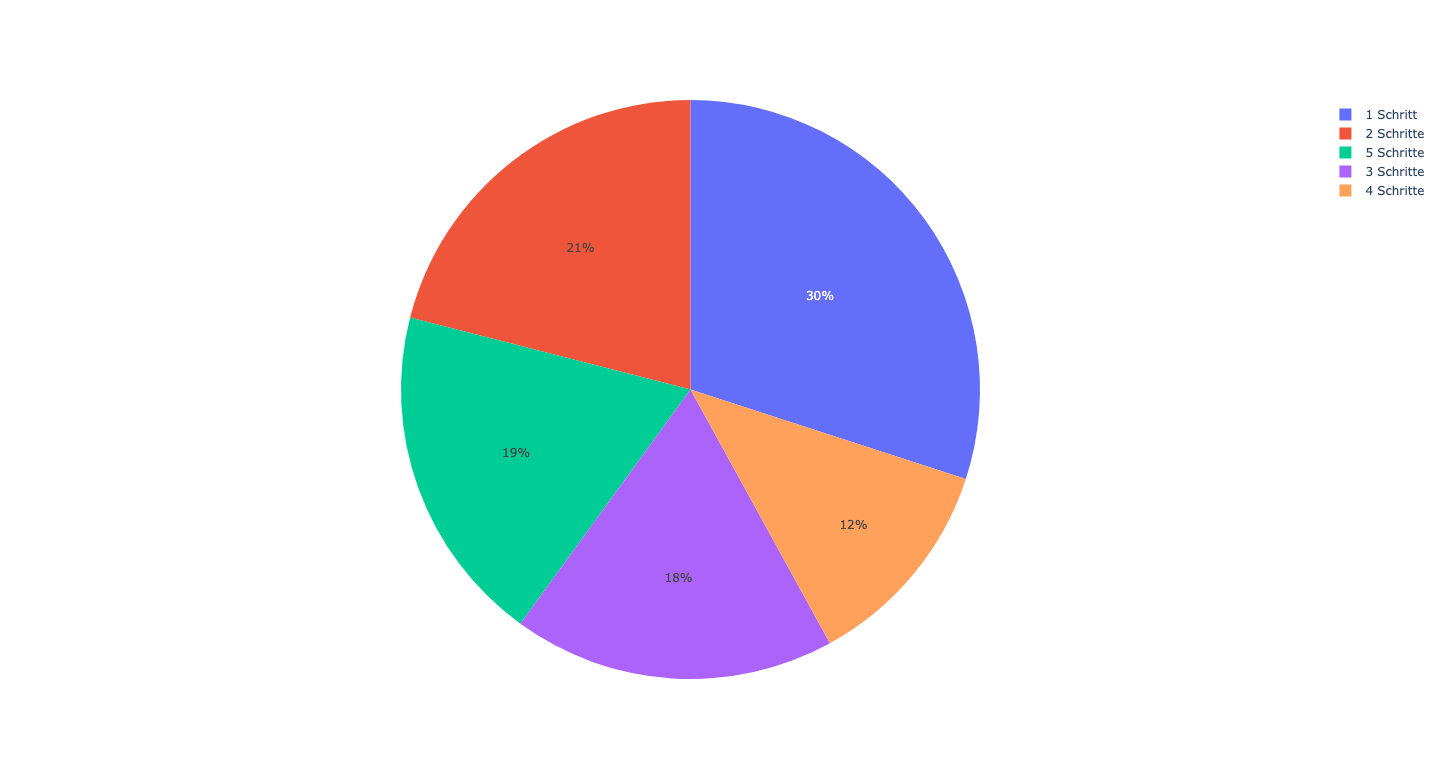
\includegraphics[width=0.85\textwidth]{gfx/Abbildungen/Startpopulation.png}
    \caption{Verteilung der Obfuskationslängen}
    \label{fig:startpopulation}
\end{figure}